\appendix
\section{Details}
\begin{itemize}
\item \cheng{Show the set of POI categories} \\
      Edinburgh: Cultural, Entertainment, Historical, Museum, Park, Structure \\
      Glasgow: Education, Museum, Park, Religion, Shopping, Structure, Transport \\
      Melbourne: City precincts, Entertainment, Institutions, Parks and spaces, Public galleries, Shopping,
                 Sports stadiums, Structures, Transport \\
      Osaka: Amusement, Entertainment, Historical, Park \\
      Toronto: Amusement, Beach, Cultural, Shopping, Sport, Structure
      The categories of POIs are shown in figure \ref{fig:poicats}.
      \begin{figure}
      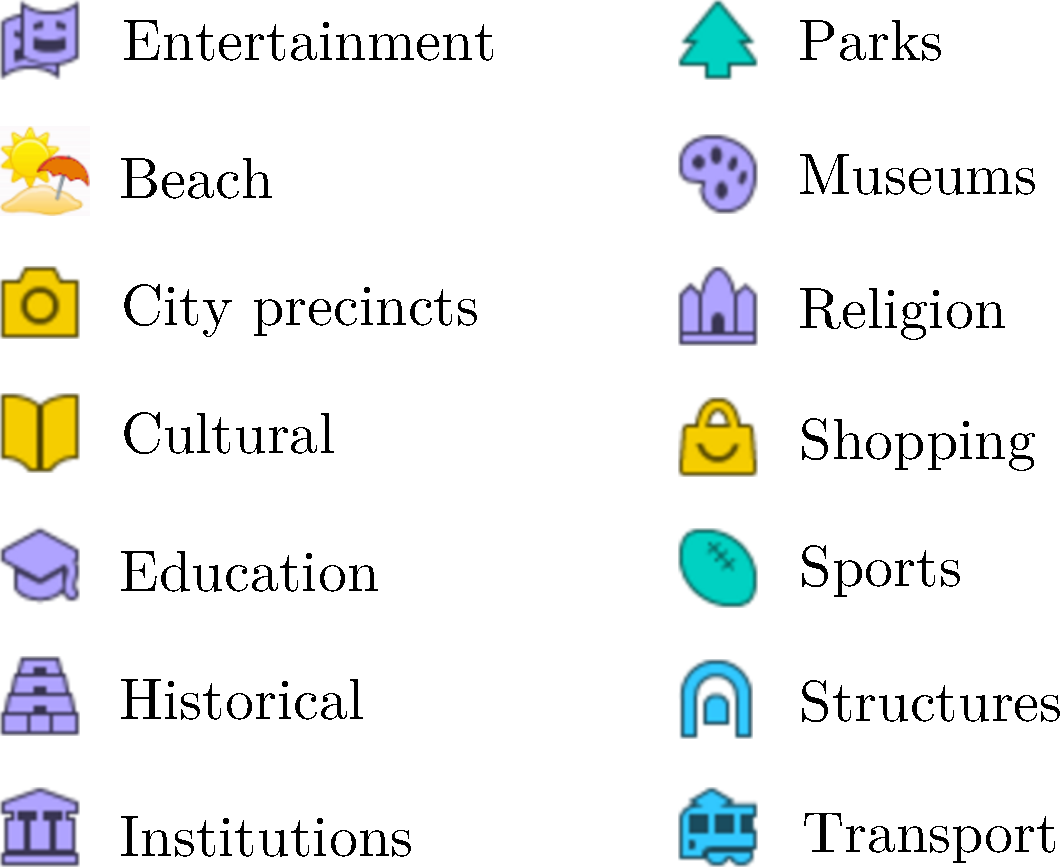
\includegraphics[width=\columnwidth]{fig/poi_cats.pdf}
      \caption{POI categories}
      \label{fig:poicats}
      \end{figure}
\item The distribution of POI popularity is shown in figure \ref{fig:popularity}.
      \begin{figure*}
      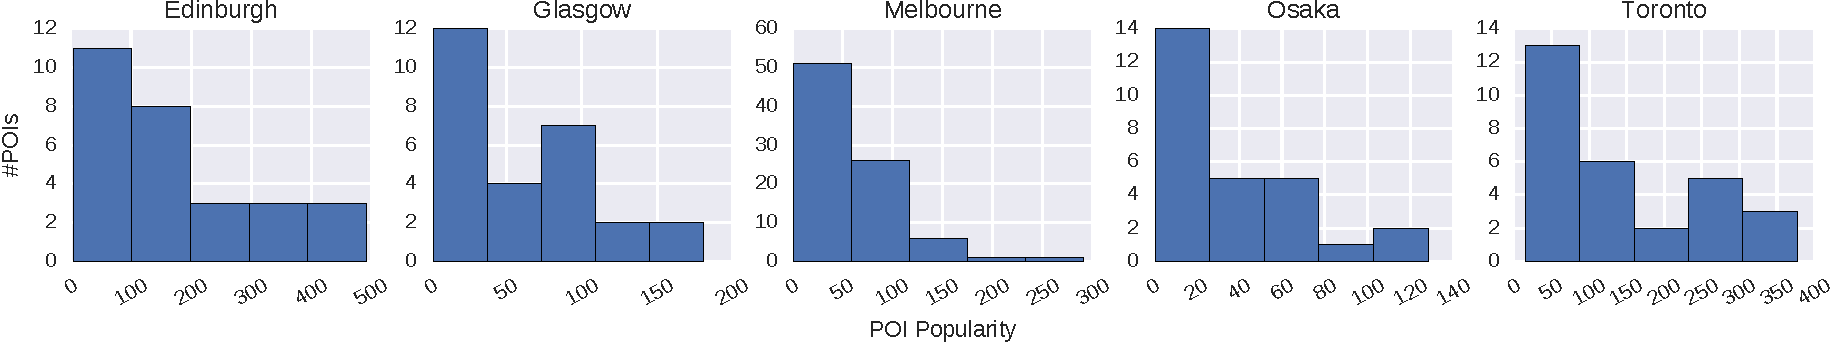
\includegraphics[width=\textwidth]{fig/poi_popularity.pdf}
      \caption{Distribution of POI popularity}
      \label{fig:popularity}
      \end{figure*}
\item The distribution of the number of visit at POI is shown in figure \ref{fig:nvisit}.
      \begin{figure*}
      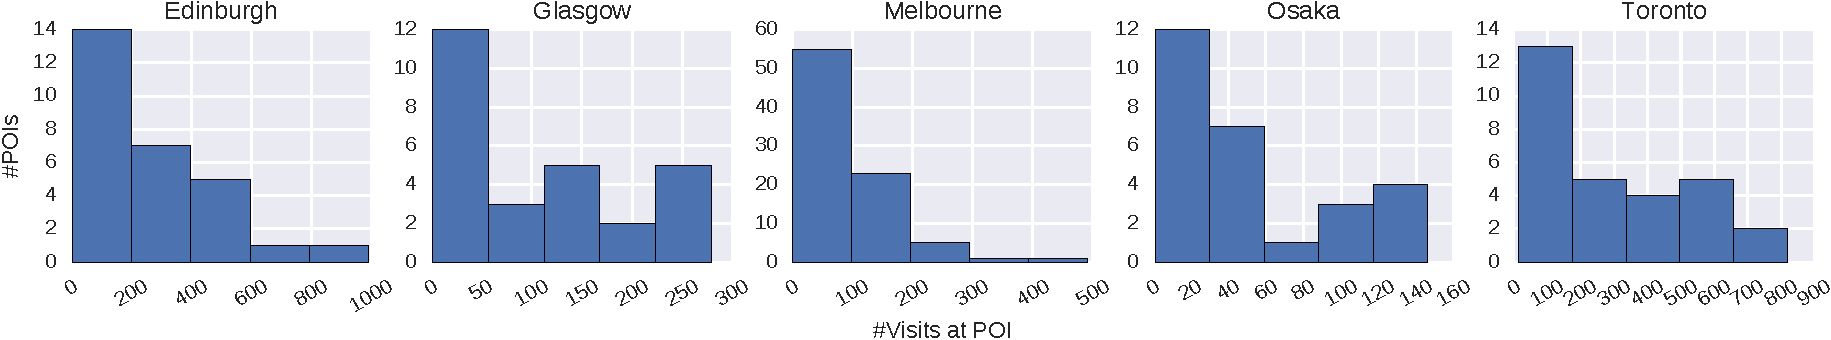
\includegraphics[width=\textwidth]{fig/poi_nvisit.pdf}
      \caption{Distribution of the number of visit at POI}
      \label{fig:nvisit}
      \end{figure*}
\item The distribution of POI visit duration is shown in figure \ref{fig:duration}.
      \begin{figure*}
      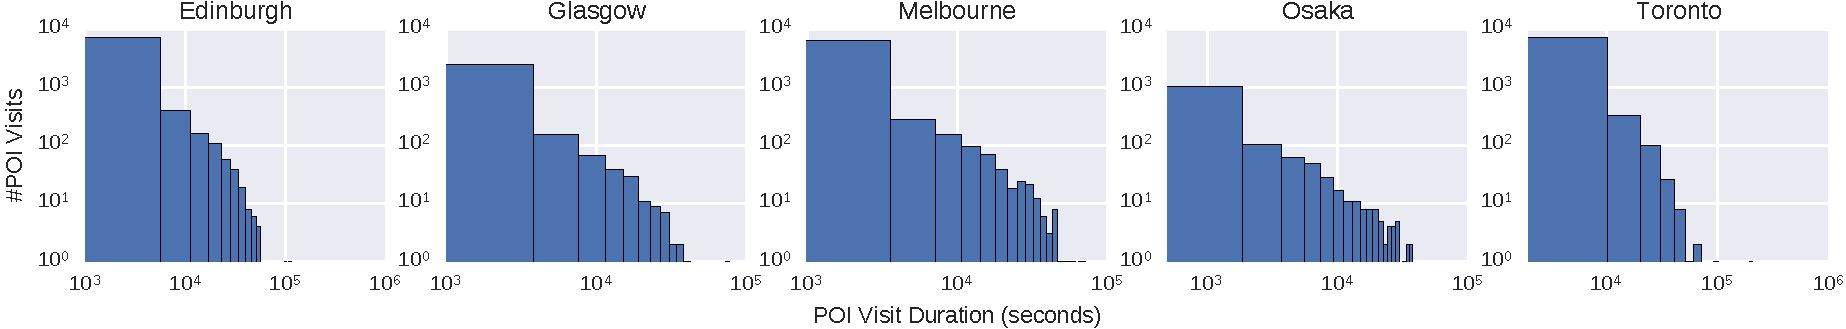
\includegraphics[width=\textwidth]{fig/visit_duration.pdf}
      \caption{Distribution of POI visit duration}
      \label{fig:duration}
      \end{figure*}
\item Heat map of POI transition matrix factorised according to $5$ POI features is shown in figure \ref{fig:transmat}
      \begin{figure*}
      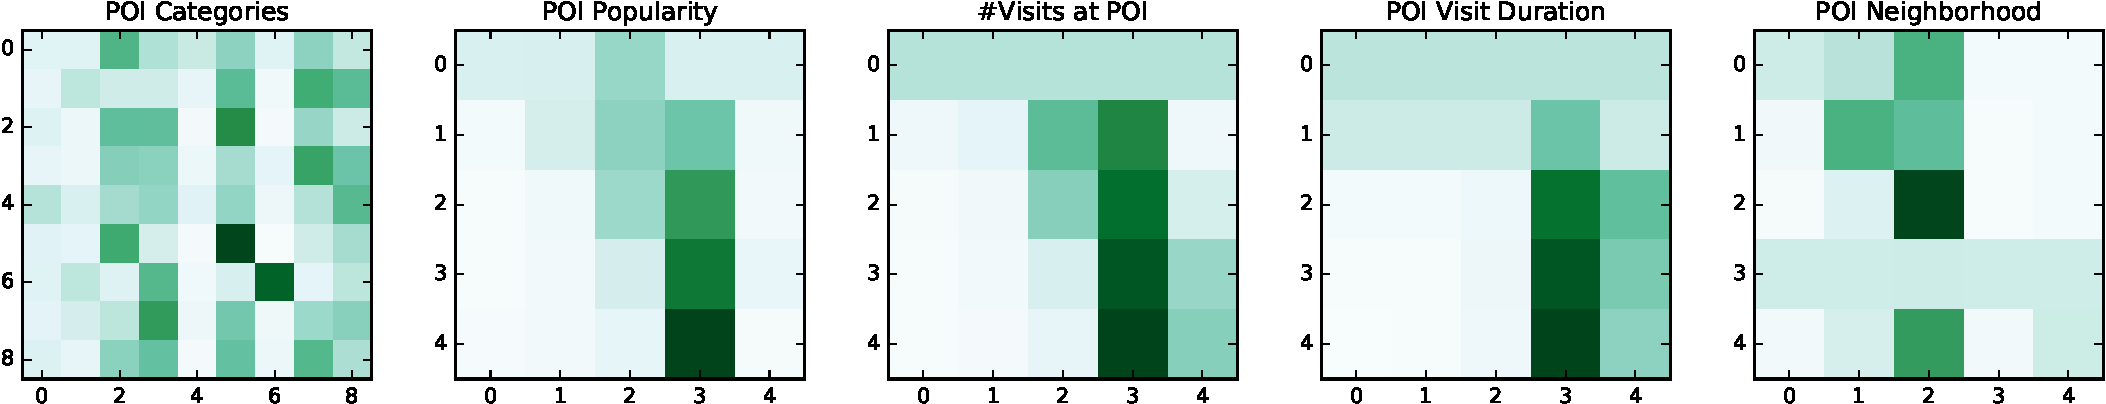
\includegraphics[width=\textwidth]{fig/poi_transmat.pdf}
      \caption{POI transition matrix factorised according to $5$ POI features (Melbourne)}
      \label{fig:transmat}
      \end{figure*}
\item There are about $12$\% of trajectories in Melbourne dataset that were failed to be evaluated
      using \textsc{PersTour} due to the timeout of integer programming solver, the timeout is $2$ hours.
\end{itemize}


\section{POIs with same features}


By computing the Kronecker product of transition matrices of all the POI features,
we get an unnormalised transition matrix of POI features.
However, to obtain the transition probabilities between each POI pair $(p_i, p_j)$,
there are two cases needs to be dealt with properly:
\begin{enumerate}
\item POI features which represent POIs that do not exist in $\mathcal{P}$,
\item POI features that corresponds to more than one POIs in $\mathcal{P}$.
\end{enumerate}

% deal with feature vector without corresponding POI or with more than one POIs.
For the first case,
the corresponding rows and columns in the result matrix of Kronecker product are simply removed.

The second case was a bit subtle.
Let POIs with exactly the same features be a POI group,
the transition probabilities associated with POIs in the same group are computed as follows:
\begin{itemize}
\item The incoming (unnormalised) transition probability of the group was divided uniformly among POIs
      in the same group, which is equivalent to choose a POI in the group uniformly at random;
\item The outgoing (unnormalised) transition probability of each POI should be the same as the
      outgoing transition probability of the POI group, as one had already been in the POI group in this case;
\item The self-loop of the POI group represents the transitions between POIs in the same group,
      suppose the (unnormalised) transition probability from a POI group to itself is $P_o$,
      and the number of POIs in the group is $N_o$,
      the transition probability from $p_i$ to $p_j$ in the same group is
      \begin{displaymath}
          P(p_j | p_i) =
          \begin{cases}
              \hfill 0, \hfill & i = j \\
              \hfill \frac{P_o}{N_o - 1}, \hfill & i \ne j \\
          \end{cases}
      \end{displaymath}
\end{itemize}
Finally, the unnormalised outgoing transition probabilities of each POI were normalized to form
a valid probability distribution
\footnote{Note that dealing with the second case before or after the normalization leads to
the same transition probabilities, which can be easily proved. \cheng{Show proof}}.


\section{Implementation details}

pyStruct, Gurobi, etc.
